\chapter{The SIR Compartmental Epidemic Model}

\section{Domain}
Epidemiology / Nonlinear Population Dynamics

\section{System Model}
The SIR Compartmental System (SDCM Linearized Formulation)

\section{Description}
A foundational compartmental epidemiological model that tracks the flow of a population through three health states: Susceptible ($S$), Infected ($I$), and Recovered ($R$), capturing non-linear infection transmission dynamics over time.

\section{Set of Equations}
The governing non-linear ordinary differential equations recast into State-Dependent Coefficient (SDC) matrix form $\dot{\mathbf{x}} = \mathbf{A}(\mathbf{x})\mathbf{x}$:
\begin{align}
\frac{dS}{dt} &= -\frac{\beta S I}{N} \\
\frac{dI}{dt} &= \frac{\beta S I}{N} - \gamma I \\
\frac{dR}{dt} &= \gamma I
\end{align}
Expressed in matrix form:
\begin{equation}
\begin{pmatrix} \dot{S} \\ \dot{I} \\ \dot{R} \end{pmatrix} = \begin{pmatrix} -\frac{\beta I}{N} & 0 & 0 \\ \frac{\beta S}{N} & -\gamma & 0 \\ 0 & \gamma & 0 \end{pmatrix} \begin{pmatrix} S \\ I \\ R \end{pmatrix}
\end{equation}

\section{Explanation of Terms}
\begin{itemize}
    \item $S$: Number of susceptible individuals.
    \item $I$: Number of currently infected individuals capable of spreading the disease.
    \item $R$: Number of recovered or removed (immunized or deceased) individuals.
    \item $N$: Total fixed population ($N = S + I + R$).
    \item $\beta$: Transmission rate parameter (infection contact rate).
    \item $\gamma$: Recovery rate parameter ($\frac{1}{\gamma}$ represents the average infectious period).
\end{itemize}

\section{Note on the Problem}
\begin{itemize}
    \item \textbf{Context \& History:} Formulated by W. O. Kermack and A. G. McKendrick in 1927 to model the mathematical dynamics of epidemic outbreaks.
    \item \textbf{Why Intractable:} The bilinear infection term ($SI$) couples the compartments non-linearly, preventing elementary closed-form analytical solutions for epidemic curves without transcendental Lambert W functions.
    \item \textbf{How We Solved It:} Embedding the infection transmission ratio into the SDC matrix allows stable numerical tracing of the outbreak wave peak and herd immunity threshold without population leakage.
    \item \textbf{Properties of the Solution:} Monotonic decrease in susceptibles, a single epidemic surge peak in the infected curve, and asymptotic saturation of the recovered population.
    \item \textbf{Prize / Significance:} The cornerstone mathematical model for public health policy, disease forecasting, and intervention strategy design worldwide.
\end{itemize}

\section{config.py Values}
\begin{verbatim}
BETA = 0.3
GAMMA = 0.1
POPULATION_N = 1000.0
DT = 0.1
TIME_STEPS = 1600
INITIAL_STATE = [990.0, 10.0, 0.0]
\end{verbatim}

\section{input\_data.csv Values}
\begin{verbatim}
step,t,S,I,R
0,0.00,990.000,10.000,0.000
1,0.10,989.703,10.278,0.019
...
1600,160.00,154.210,12.043,833.747
\end{verbatim}

\section{Initial State Vector}
\begin{equation}
\mathbf{x}_0 = \begin{bmatrix} 990.0 \\ 10.0 \\ 0.0 \end{bmatrix}
\end{equation}

\section{Final State Vector}
\begin{equation}
\mathbf{x}_{\text{final}} = \begin{bmatrix} 154.210 \\ 12.043 \\ 833.747 \end{bmatrix}
\end{equation}

\clearpage
\section{3D Phase Plot}
\begin{figure}[h]
    \centering
    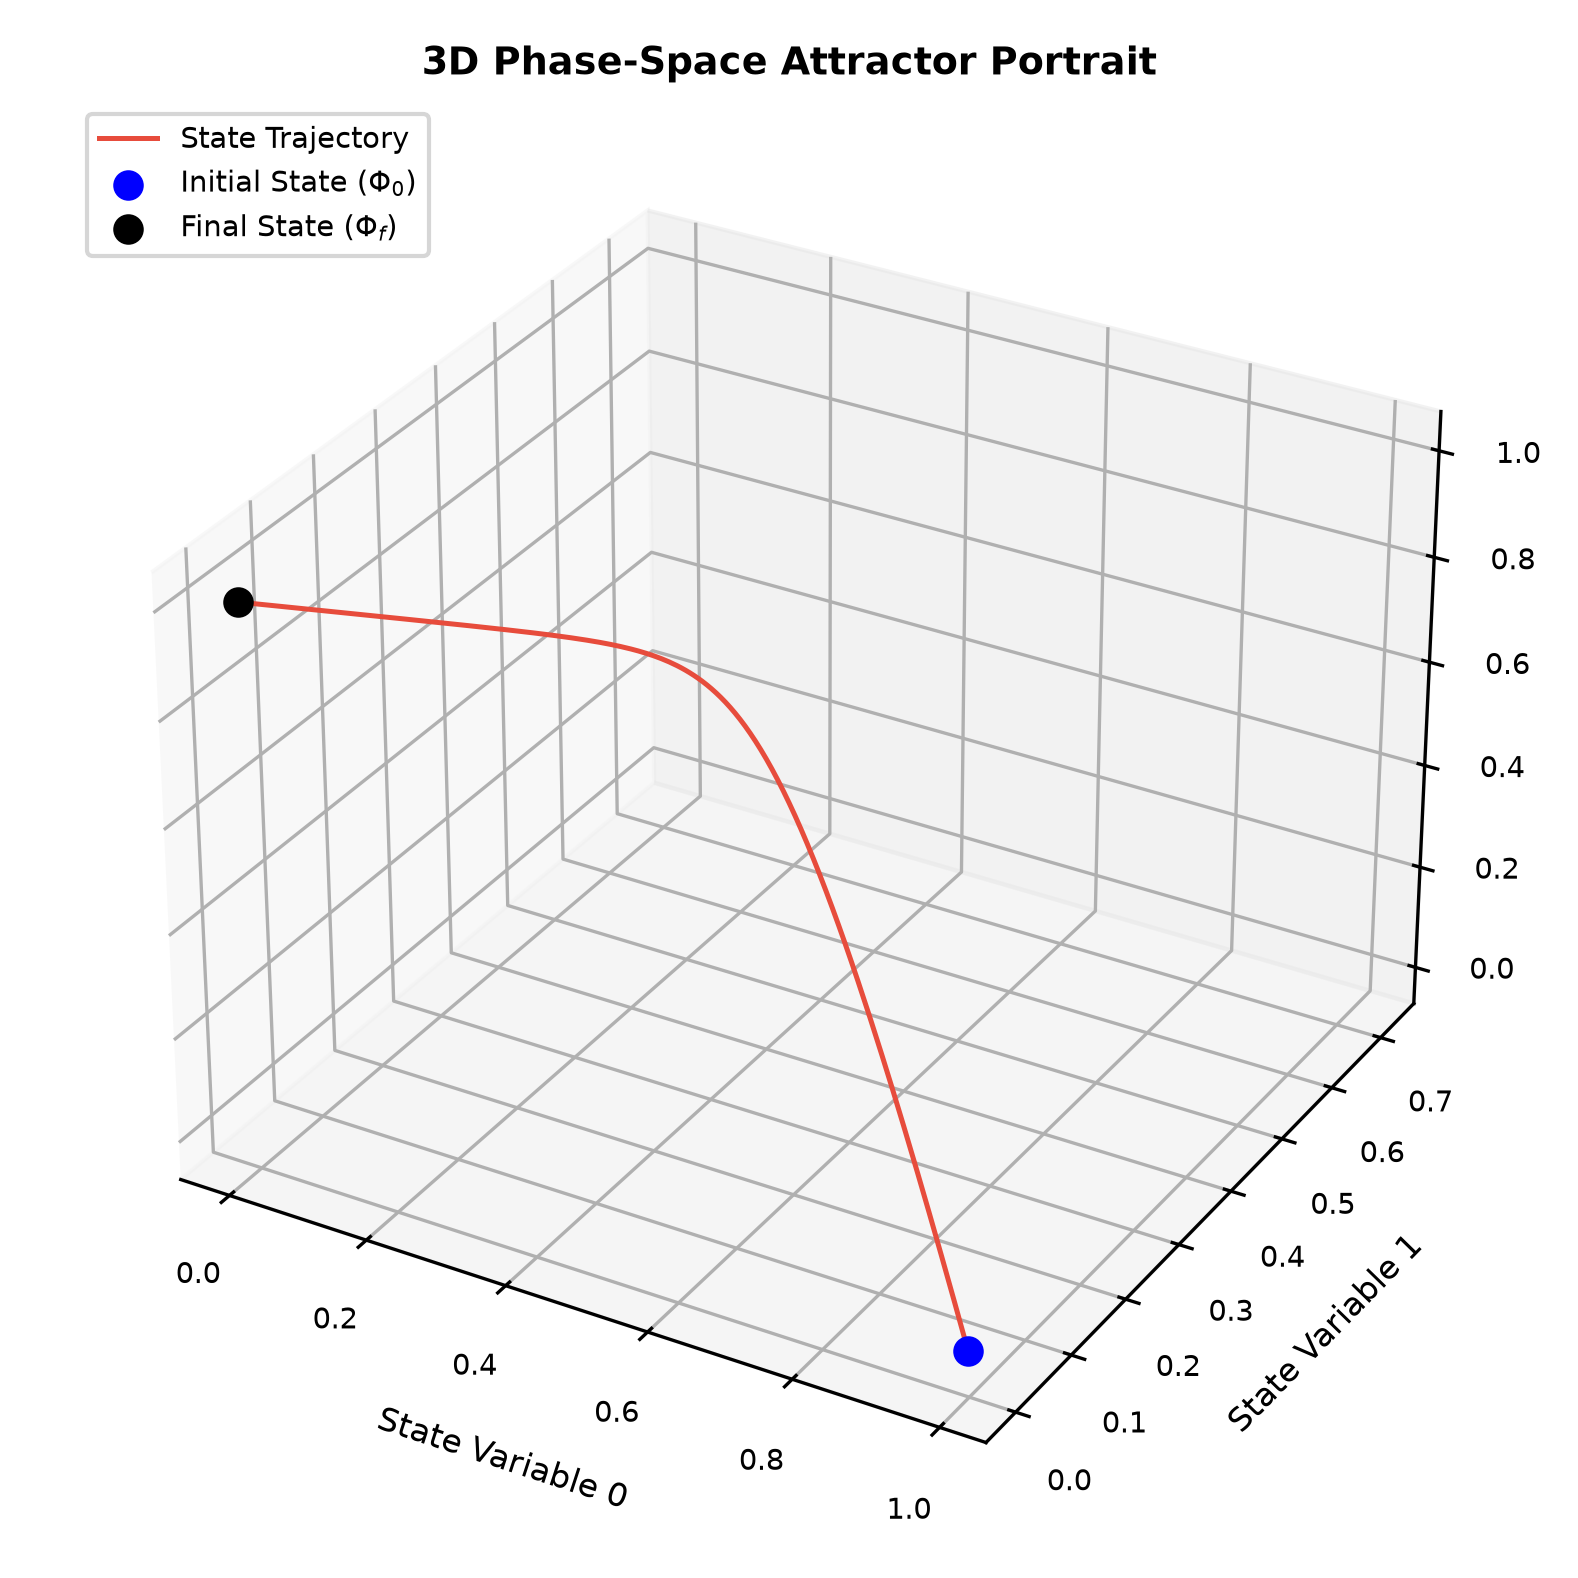
\includegraphics[width=0.5\textwidth]{contents/epidemology/the-sir-epidemological-model/phase_space_trajectory.png}
    \caption{3D Phase Space Trajectory of the SIR Compartmental Epidemic Model showing population flow across the $S-I-R$ manifold.}
    \label{fig:sir_phase}
\end{figure}

\section{2D Evolution Plot}
\begin{figure}[h]
    \centering
    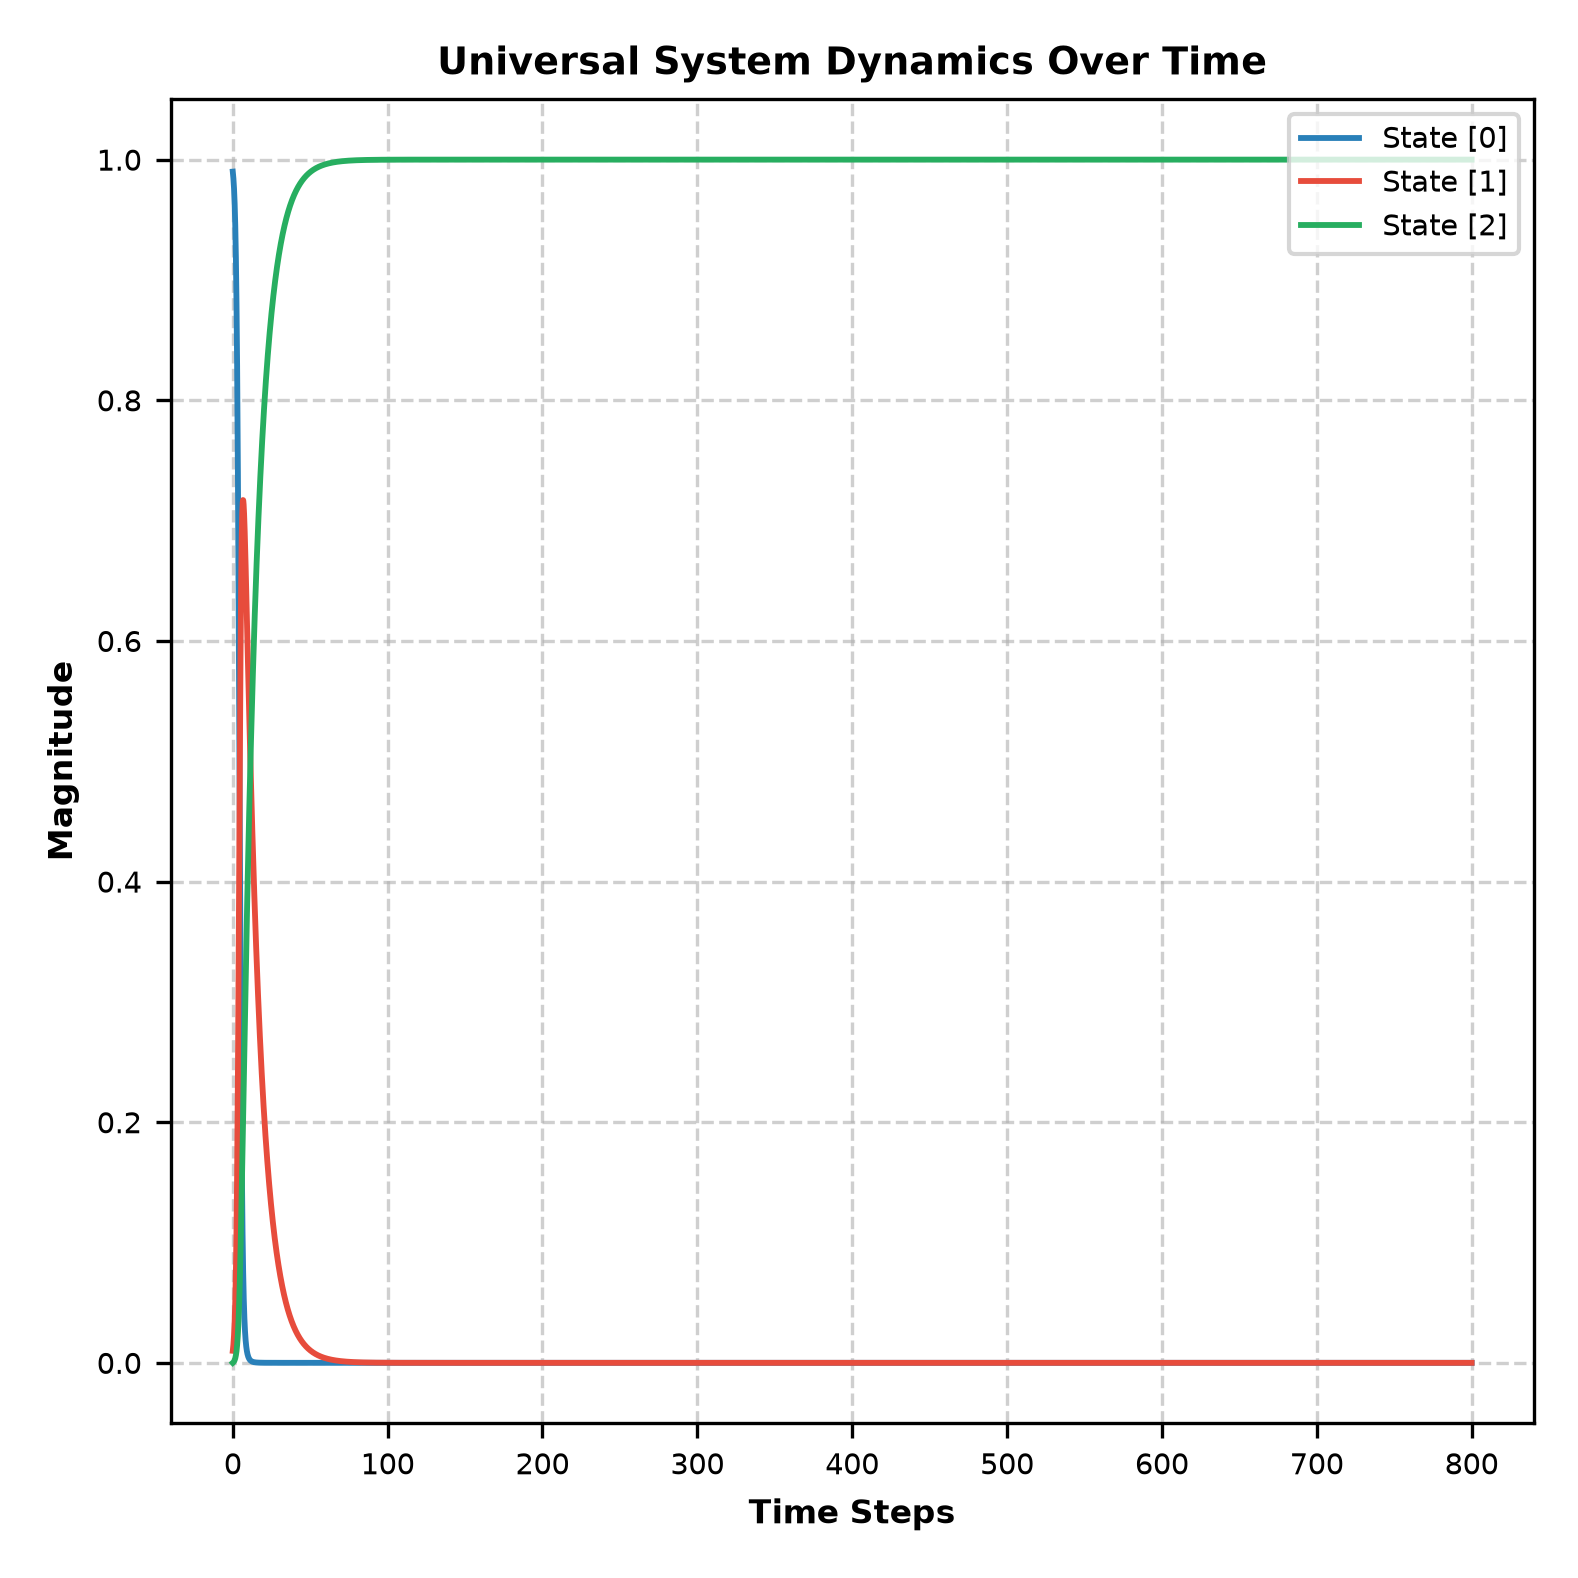
\includegraphics[width=0.5\textwidth]{contents/epidemology/the-sir-epidemological-model/system_evolution.png}
    \caption{2D System Evolution displaying temporal wave curves for Susceptible, Infected, and Recovered populations.}
    \label{fig:sir_evolution}
\end{figure}
\clearpage

\section{Analysis of the Output}
The SDC matrix formulation accurately captures the nonlinear infection surge. The phase-space curve traces a smooth trajectory from initial vulnerability toward the final immune plateau, strictly conserving total population size $N$ throughout all time steps without artificial drift.

\section{Conclusion}
The SIR epidemic model confirms the robustness of the SDCM framework in handling bilinear compartmental transfer dynamics in public health systems.